\documentclass[11pt, oneside]{article}

\usepackage[english]{babel}
\usepackage[utf8]{inputenc}
\usepackage{amsmath}
\usepackage{graphicx}
\usepackage[colorinlistoftodos]{todonotes}
\usepackage{pslatex}
\usepackage[margin=1in]{geometry}
\usepackage{listings}
\usepackage{color}
\usepackage[margin=.25in]{caption}
\usepackage{subcaption}
\usepackage{tikz}
\usepackage{pgfplots}
\usepackage{verbatim}
\usetikzlibrary{automata,topaths}
\definecolor{mygreen}{rgb}{0,0.6,0}
\definecolor{mygray}{rgb}{0.5,0.5,0.5}
\definecolor{mymauve}{rgb}{0.58,0,0.82}

\lstset{ %
  backgroundcolor=\color{white},   % choose the background color
  basicstyle=\footnotesize,        % size of fonts used for the code
  breaklines=true,                 % automatic line breaking only at whitespace
  captionpos=b,                    % sets the caption-position to bottom
  commentstyle=\color{mygreen},    % comment style
  escapeinside={\%*}{*)},          % if you want to add LaTeX within your code
  keywordstyle=\color{blue},       % keyword style
  stringstyle=\color{mymauve},     % string literal style
}


\title{HODOR: HODOR On-Disk Orthogonal Range-trees}

\author{Stephanie Wang (swang93@mit.edu)\\
Bennett Cyphers (bcyphers@mit.edu)\\
Katie Siegel (ksiegel@mit.edu)\\[2ex]
6.851 Final Report}

\date{\today}

\begin{document}

\maketitle
\clearpage

\section{Introduction}

Many web applications today require data queries in two or more dimensions. For instance, a point of interest on a map has latitude and longitude coordinates, and may be indexed by other comparable values. These include start and end times for an event, price ranges for a business, or average user rating for a service. Databases typically support efficient range querying on one primary key at a time. Multi-dimensional range queries, however, are expensive and require several linear passes of the dataset in most implementations. On the other hand, orthogonal range trees with fractional cascading can improve range queries in $d$ dimensions to $O(\log^{d-1} n + k)$ time, where $k$ is the size of the result set [CITATION]. 

In-memory orthogonal range tree implementations have been able to achieve significant query time speedup [CITATION, Tim's paper]. These can be used to extend a database for smaller datasets. Most datasets, however, are too large to fit in memory, and therefore require an on-disk implementation. To this end, we present HODOR, an on-disk Python implementation of range-trees. 

The main obstacle in an on-disk implementation of orthogonal range trees is the added overhead in disk access time. Therefore, in this paper, we explore different methods of optimizing disk I/O accesses. First, we present optimizations on the range tree structure itself. Second, we propose methods of optimizing individual node serialization. Third, we explore optimizing the serialization of the entire tree. Finally, we present results from benchmarking these optimizations against a Python database [BUZHUG CITATION]. 


\section{Data Structure}


Ordinarily, multidimensional range queries are expensive, with most methods taking $O(n)$ time. With large databases, a runtime of $O(n)$ is highly costly. To allow for polylog time range queries, we implemented an orthogonal range tree, generalized to d dimensions. We used a B+ tree for our implementation, as B+ trees are more efficient given the architecture of our machine. In this section, we discuss these data structures and the resulting speedup.

\subsection{B+ Tree-Based Orthogonal Range Tree}
B trees are commonly used for databases, they optimize for the number of disk accesses made for queries. B+ trees are extensions to B trees in which all data is stored in the leaves, and each leaf keeps a pointer to its successor. B+ trees maintain a search time of $O(\log_B n)$. We extend this B+ tree structure to form the orthogonal range tree.

An orthogonal range tree is an extension to a B+ tree in which each node in the tree points to a tree containing the contents of the node's subtree sorted in the next dimension. Dimensions are ordered hierarchically, with the "top level" dimension corresponding to the first-level tree, the second  dimension's information held in subtrees of the nodes in that tree, and so on. B trees support queries in time $O(\log_B^d n + k)$, where $d$ is the number of dimensions of the data. Because we optimize for query time, orthogonal range trees do add a factor of overhead for additional data storage; this space overhead factor is $O(\log_B^{d-1} n)$.   
	
\subsection{Using the data structure}
The tree is constructed in preprocessing, which takes $O(n \cdot \log_B^{d-1} n)$ time. The user can specify any d dimensions for the dataset to be indexed on.
A dimension can be any continuous, comparable data type which can be mapped to a number.
Searches are performed on ranges for any subset of the d dimensions, by passing the range tree a set of {dimension: (range start, range end)} pairs. Open-ended range queries are not explicitly supported, but can be performed in practice by setting one of the range bounds to $\pm\infty$.




\section{Introduction}
Goals:
	I/O Optimization
    


\section{Implementation}

In python
serializer


\section{Optimization methods}

\subsection{B trees}


\subsection{Node serialization}

In order to store range trees on disk, we require an efficient method to
serialize and deserialize the data structure. In Hodor, we represent a Python
\texttt{RangeTree} instance as a list of serialized nodes, which may be
instances of \texttt{RangeNode} or \texttt{RangeLeaf}. This list is stored in a
``tree file", which can be written to and read by a \texttt{Serializer} class. 

During preprocessing, when building the tree from datapoints,
\texttt{Serializer} is initialized in write mode to build the tree file.
\texttt{Serializer} in write mode exposes a \texttt{dumps(node)} method that
takes in a node instance, serializes the node, and appends it to the tree file.
This method also assigns the node instance a pointer into the tree file, which
is the number of nodes appended previously to it. 

Once the tree is fully built, we call \texttt{Serializer.flush()}, which
flushes the tree file to disk. From this point onwards, \texttt{Serializer} can
be used to read the tree.

In read mode, \texttt{Serializer.loads(pointer)} can be called to deserialize a
single node into a Python node instance, given its pointer into the tree file.
So, to load the child of a node instance, we simply store the child's tree file
pointer as an attribute of the parent. \texttt{loads} is implemented by seeking
the pointer in the tree file and reading out a single node's worth of bytes.

% maybe some of this should go into Implementation details maybe something
% about cPickle vs struct
The seeking method varies by serializer. In Hodor, we test two main node
serialization methods. The first is using a delimiter, such as a newline
character, between nodes. This is convenient because it allows us to support
arbitrarily sized datapoint values. In addition, Python is able to perform
specific line reads quickly, by using either an iterator on the file or a
linecache [CITATION, f.lines() iterator, linecache]. 

The second method we use is to pack nodes into fixed-length strings, which we
call ``blocks". Each node in a range tree stores a constant number of values,
including min, max, and child pointers. This allows us to serialize each node
as a block, as long as we know the maximum sizes of these values. The block
method makes seeking efficient because it allows us to calculate exact offsets
between \texttt{Serializer}'s current byte position in the file and a given
node's pointer. However, this method also limits the amount and type of data
that can be stored at each node. 

\subsection{Tree serialization}

\begin{figure}[p]
    \centering
    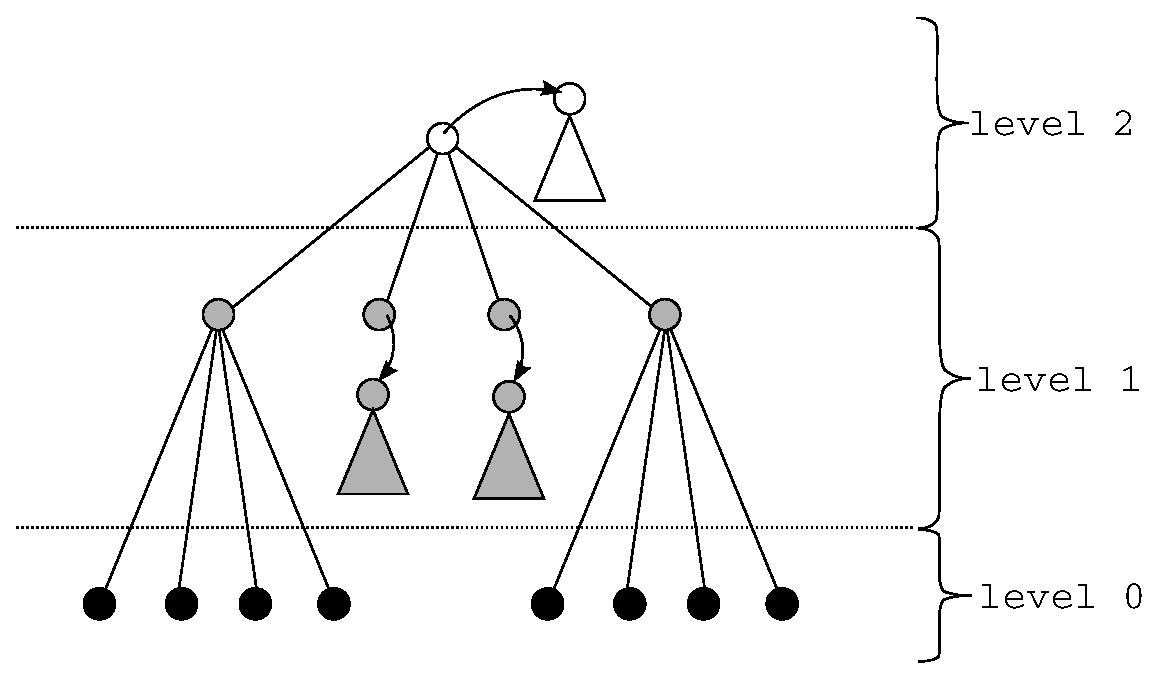
\includegraphics[width=0.8\textwidth]{fig1.eps}
    \caption{Awesome Image}
\end{figure}
\begin{figure}[p]
    \centering
    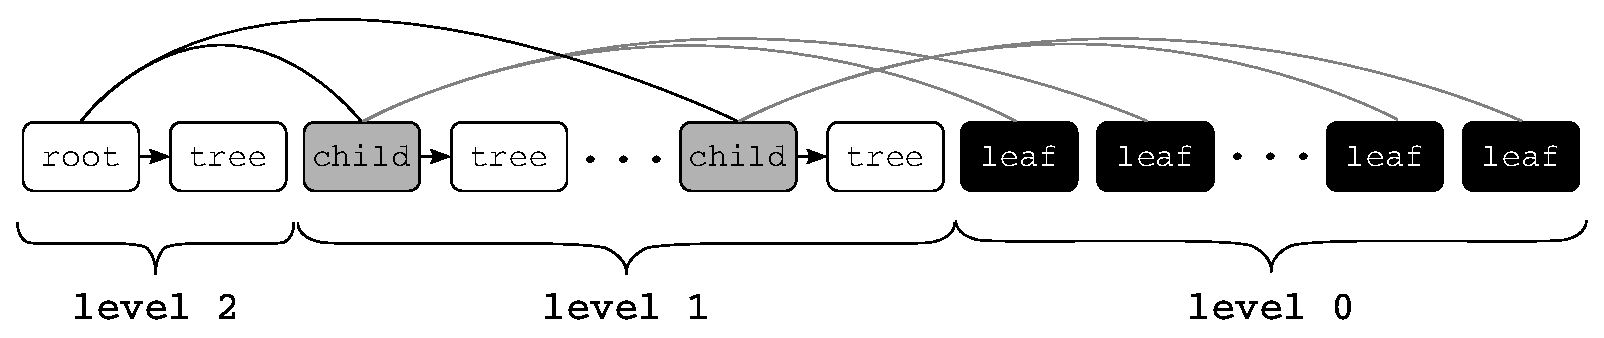
\includegraphics[width=0.8\textwidth]{fig2.eps}
    \caption{Awesome Image}
\end{figure}

\section{Results}

We found and formatted two major data sets of two different sizes. The first data set corresponds to New York City parking garages, and the second data set contains entries for every documented instance of crime in the city of Chicago since the year 2001. The second data set is two orders of magnitude larger than the first data set. Both data sets contain multiple numeric fields apart from location on which range queries may be performed. We analyzed the performance of the altered Buzhug database by performing a wide variety of range queries and examining the performance gains.


\section{Analysis}

\subsection{Total Time}

\subsection{Disk Reads}

\section{Conclusion}


\section{References}

\noindent

\begin{description}

\item item

\end{description}
\end{document}
